%Chapter 1
\chapter{Introduction and background}  %J.H Marais, C.J.R. Kriel
\pagenumbering{arabic} 
\setcounter{page}{1}
\vspace{38em}

\hrulefill
\\
\enquote*{\textit{Your ideas are like diamonds. Without the refining process they are just rock. But cutting away impurities, they become priceless.}} - Paul Kearly\\
\newpage


\section{Preamble}

\section{Background on deep level mining}

\subsection{Mining profitability}
 Various technical, economic, social and operational challenges are posing a risk to the profitability of the South African mining sector. One of the challenges the sector faces  is a rise in the cost of operation\cite{neingo2016trends}.\par
%\paragraph*{Falling ore grades}\leavevmode\\
A considerable factor that is contributing the the rise of operational costs in South African gold mines has been the increase in electricity costs. As shown in figure \ref{fig: Eskom tariffs} the general cost of electricity has increased at a rate greater than inflation since 2008 \cite{Eskom2013Tariffs}.
\begin{figure}[h]
	\centering
	\fbox{% GNUPLOT: LaTeX picture with Postscript
\begingroup
  \makeatletter
  \providecommand\color[2][]{%
    \GenericError{(gnuplot) \space\space\space\@spaces}{%
      Package color not loaded in conjunction with
      terminal option `colourtext'%
    }{See the gnuplot documentation for explanation.%
    }{Either use 'blacktext' in gnuplot or load the package
      color.sty in LaTeX.}%
    \renewcommand\color[2][]{}%
  }%
  \providecommand\includegraphics[2][]{%
    \GenericError{(gnuplot) \space\space\space\@spaces}{%
      Package graphicx or graphics not loaded%
    }{See the gnuplot documentation for explanation.%
    }{The gnuplot epslatex terminal needs graphicx.sty or graphics.sty.}%
    \renewcommand\includegraphics[2][]{}%
  }%
  \providecommand\rotatebox[2]{#2}%
  \@ifundefined{ifGPcolor}{%
    \newif\ifGPcolor
    \GPcolortrue
  }{}%
  \@ifundefined{ifGPblacktext}{%
    \newif\ifGPblacktext
    \GPblacktextfalse
  }{}%
  % define a \g@addto@macro without @ in the name:
  \let\gplgaddtomacro\g@addto@macro
  % define empty templates for all commands taking text:
  \gdef\gplbacktext{}%
  \gdef\gplfronttext{}%
  \makeatother
  \ifGPblacktext
    % no textcolor at all
    \def\colorrgb#1{}%
    \def\colorgray#1{}%
  \else
    % gray or color?
    \ifGPcolor
      \def\colorrgb#1{\color[rgb]{#1}}%
      \def\colorgray#1{\color[gray]{#1}}%
      \expandafter\def\csname LTw\endcsname{\color{white}}%
      \expandafter\def\csname LTb\endcsname{\color{black}}%
      \expandafter\def\csname LTa\endcsname{\color{black}}%
      \expandafter\def\csname LT0\endcsname{\color[rgb]{1,0,0}}%
      \expandafter\def\csname LT1\endcsname{\color[rgb]{0,1,0}}%
      \expandafter\def\csname LT2\endcsname{\color[rgb]{0,0,1}}%
      \expandafter\def\csname LT3\endcsname{\color[rgb]{1,0,1}}%
      \expandafter\def\csname LT4\endcsname{\color[rgb]{0,1,1}}%
      \expandafter\def\csname LT5\endcsname{\color[rgb]{1,1,0}}%
      \expandafter\def\csname LT6\endcsname{\color[rgb]{0,0,0}}%
      \expandafter\def\csname LT7\endcsname{\color[rgb]{1,0.3,0}}%
      \expandafter\def\csname LT8\endcsname{\color[rgb]{0.5,0.5,0.5}}%
    \else
      % gray
      \def\colorrgb#1{\color{black}}%
      \def\colorgray#1{\color[gray]{#1}}%
      \expandafter\def\csname LTw\endcsname{\color{white}}%
      \expandafter\def\csname LTb\endcsname{\color{black}}%
      \expandafter\def\csname LTa\endcsname{\color{black}}%
      \expandafter\def\csname LT0\endcsname{\color{black}}%
      \expandafter\def\csname LT1\endcsname{\color{black}}%
      \expandafter\def\csname LT2\endcsname{\color{black}}%
      \expandafter\def\csname LT3\endcsname{\color{black}}%
      \expandafter\def\csname LT4\endcsname{\color{black}}%
      \expandafter\def\csname LT5\endcsname{\color{black}}%
      \expandafter\def\csname LT6\endcsname{\color{black}}%
      \expandafter\def\csname LT7\endcsname{\color{black}}%
      \expandafter\def\csname LT8\endcsname{\color{black}}%
    \fi
  \fi
    \setlength{\unitlength}{0.0500bp}%
    \ifx\gptboxheight\undefined%
      \newlength{\gptboxheight}%
      \newlength{\gptboxwidth}%
      \newsavebox{\gptboxtext}%
    \fi%
    \setlength{\fboxrule}{0.5pt}%
    \setlength{\fboxsep}{1pt}%
\begin{picture}(9360.00,4032.00)%
    \gplgaddtomacro\gplbacktext{%
      \colorrgb{0.00,0.00,0.00}%
      \put(682,1144){\makebox(0,0)[r]{\strut{}$0$}}%
      \colorrgb{0.00,0.00,0.00}%
      \put(682,1422){\makebox(0,0)[r]{\strut{}$5$}}%
      \colorrgb{0.00,0.00,0.00}%
      \put(682,1701){\makebox(0,0)[r]{\strut{}$10$}}%
      \colorrgb{0.00,0.00,0.00}%
      \put(682,1979){\makebox(0,0)[r]{\strut{}$15$}}%
      \colorrgb{0.00,0.00,0.00}%
      \put(682,2258){\makebox(0,0)[r]{\strut{}$20$}}%
      \colorrgb{0.00,0.00,0.00}%
      \put(682,2536){\makebox(0,0)[r]{\strut{}$25$}}%
      \colorrgb{0.00,0.00,0.00}%
      \put(682,2814){\makebox(0,0)[r]{\strut{}$30$}}%
      \colorrgb{0.00,0.00,0.00}%
      \put(682,3093){\makebox(0,0)[r]{\strut{}$35$}}%
      \colorrgb{0.00,0.00,0.00}%
      \put(682,3371){\makebox(0,0)[r]{\strut{}$40$}}%
      \colorrgb{0.00,0.00,0.00}%
      \put(814,924){\makebox(0,0){\strut{}$2006$}}%
      \colorrgb{0.00,0.00,0.00}%
      \put(2172,924){\makebox(0,0){\strut{}$2008$}}%
      \colorrgb{0.00,0.00,0.00}%
      \put(3530,924){\makebox(0,0){\strut{}$2010$}}%
      \colorrgb{0.00,0.00,0.00}%
      \put(4888,924){\makebox(0,0){\strut{}$2012$}}%
      \colorrgb{0.00,0.00,0.00}%
      \put(6246,924){\makebox(0,0){\strut{}$2014$}}%
      \colorrgb{0.00,0.00,0.00}%
      \put(7604,924){\makebox(0,0){\strut{}$2016$}}%
      \colorrgb{0.00,0.00,0.00}%
      \put(8962,924){\makebox(0,0){\strut{}$2018$}}%
    }%
    \gplgaddtomacro\gplfronttext{%
      \csname LTb\endcsname%
      \put(176,2257){\rotatebox{-270}{\makebox(0,0){\strut{}\% increase}}}%
      \put(4888,594){\makebox(0,0){\strut{}Year}}%
      \put(4888,3701){\makebox(0,0){\strut{}Electricity price increases in South Africa}}%
      \csname LTb\endcsname%
      \put(6770,393){\makebox(0,0)[r]{\strut{}Eskom general tariff increases (\%)}}%
      \csname LTb\endcsname%
      \put(1493,1562){\makebox(0,0){\strut{}6.0}}%
      \put(2172,2759){\makebox(0,0){\strut{}27.5}}%
      \put(2851,2970){\makebox(0,0){\strut{}31.3}}%
      \put(3530,2608){\makebox(0,0){\strut{}24.8}}%
      \put(4209,2664){\makebox(0,0){\strut{}25.8}}%
      \put(4888,2118){\makebox(0,0){\strut{}16.0}}%
      \put(5567,1673){\makebox(0,0){\strut{}8.0}}%
      \put(6246,1673){\makebox(0,0){\strut{}8.0}}%
      \put(6925,1673){\makebox(0,0){\strut{}8.0}}%
      \put(7604,1673){\makebox(0,0){\strut{}8.0}}%
      \put(8283,1673){\makebox(0,0){\strut{}8.0}}%
      \csname LTb\endcsname%
      \put(6770,173){\makebox(0,0)[r]{\strut{}Inflation rate in south Africa (\%)}}%
    }%
    \gplbacktext
    \put(0,0){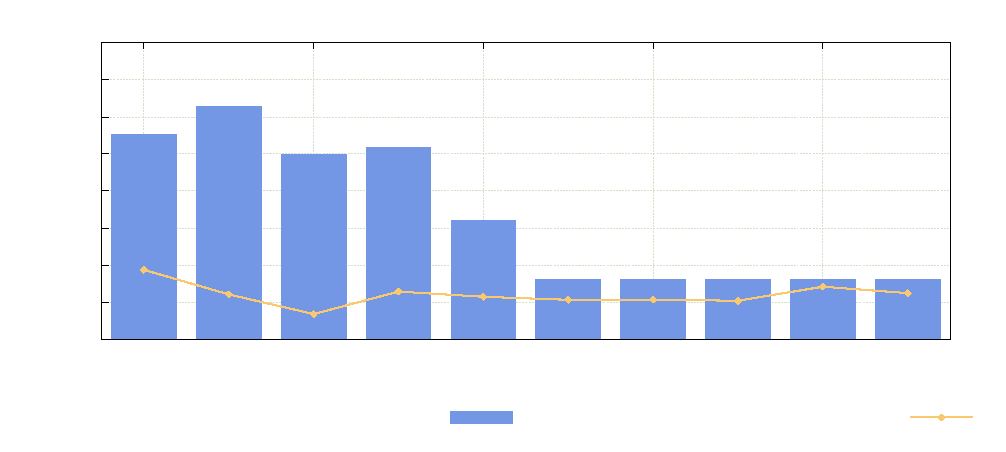
\includegraphics{Graphs/1/Eskom/Eskom}}%
    \gplfronttext
  \end{picture}%
\endgroup
}
	\caption[Electricity price increases between 2007 and 2017.]{Electricity price increases between 2007 and 2017 \cite{Eskom2013Tariffs,Inflation2013}.}
	\label{fig: Eskom tariffs}
\end{figure}
\par
In addition to rising electricity cost, gold ore grades of South African mines have fallen substantially over the last few decades\cite{mudd2007global}. As ore grades decline, the energy utilised per unit of metal increases exponentially \cite{muller2010numerical}. Therefore mines require significantly more energy per unit of metal produced. This combination of tariff increases and increased energy usage per unit  have lead to significant rises in mining operation costs. \par
%\paragraph*{Rising operational costs}\leavevmode\\

\subsection{Mining systems and energy}
The mining industry uses extensive amounts of energy. In South Africa, the industry utilizes approximately 15\% of the national electricity supplier's yearly output. Of which, gold and platinum mines use 80\%.\cite{Eskom2010Energy}\par
Figure \ref{fig: Energy Split} shows the division of energy within the mining industry. From the chart it is reasoned that energy can be reduced most effectively through implementing energy interventions on mining material handling, processing and compressed air systems.
\begin{figure}[h]
	\centering
	\fbox{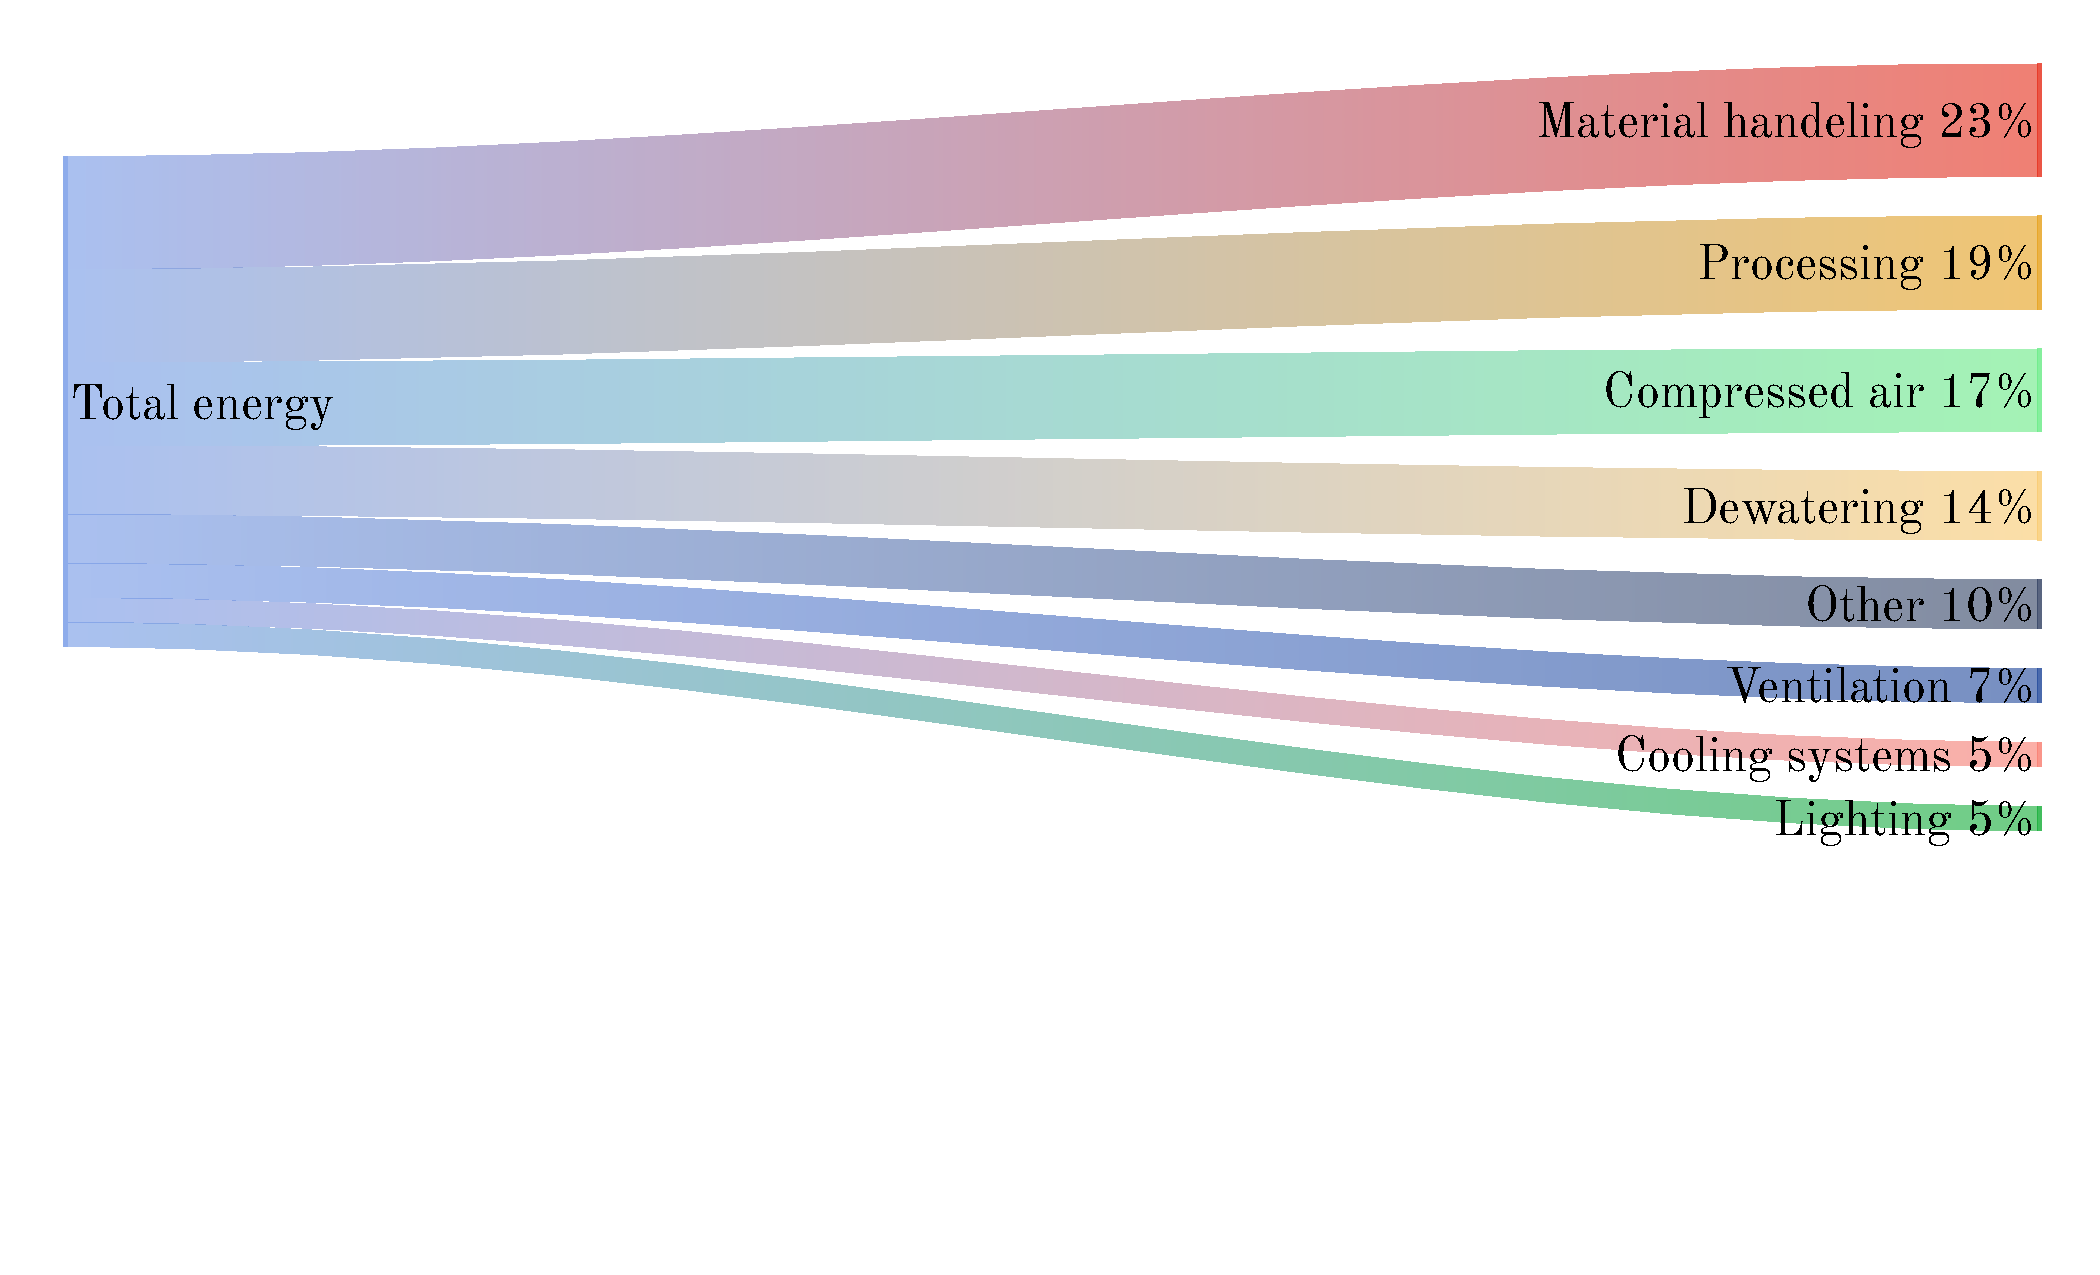
\includegraphics[ trim=0.7cm 7cm 0.7cm 0.7cm,width=\textwidth]{Graphs/1/Sankey/Sankey}}
	\caption[The energy split for the south african mining industry.]{The energy split for the south african mining industry \cite{Eskom2010Energy}.}
	\label{fig: Energy Split}
\end{figure}
\par
%\subsection{Need to improve service delivery and efficiency}
%\texttt{Discuss how improvements in service delivery and efficiency will reduce operation costs therefore increase profitability.}
\section{Mining compressed air}
Due to their reliability, versatilely and ease of use, the South African mining industry has installed extensive compressed air networks. These systems can have compressors with capacities of up to 15 \gls{mw} \cite{Marais2012PhD}.\par
However, the supply of compressed air is a highly energy demanding and costly process \cite{padachi2009energy}.  The energy used for compressed air production contributes to between 9\% and 20\% of the total mining energy consumption \cite{Eskom2010Energy,du2011development}. \par
Large compressed air systems are likely inefficient. Internationally, the expected energy savings potential of a large compressed air network is 15\% \cite{neale2009compressed}. Marais \cite{marais2013simplification} showed that energy savings of up to 30\% and 40\% can be obtained from some systems. 
\subsection{Compressed air in operation}
	\paragraph{Operation schedule}\leavevmode\\
	On a typical mine, various operations will take place at different times of the day. Depending on the activity taking place, many mines will control the pressure to meet the requirements \cite{Kriel2014Masters,Marais2012PhD}. Figure \ref{fig: Mining schedule} shows the schedule and pressure requirement on a typical deep level mine.\par 
	As shown in the figure, the pressure requirement changes depending on the activity taking place. The drilling shift typically has the highest pressure requirement whilst blasting shift requires the lowest. Schedules and operation philosophies can differ between mines. Different operational schedules require alternative pressure requirement profiles.
		\begin{figure}[h]
		\centering
		\fbox{% GNUPLOT: LaTeX picture with Postscript
\begingroup
  \makeatletter
  \providecommand\color[2][]{%
    \GenericError{(gnuplot) \space\space\space\@spaces}{%
      Package color not loaded in conjunction with
      terminal option `colourtext'%
    }{See the gnuplot documentation for explanation.%
    }{Either use 'blacktext' in gnuplot or load the package
      color.sty in LaTeX.}%
    \renewcommand\color[2][]{}%
  }%
  \providecommand\includegraphics[2][]{%
    \GenericError{(gnuplot) \space\space\space\@spaces}{%
      Package graphicx or graphics not loaded%
    }{See the gnuplot documentation for explanation.%
    }{The gnuplot epslatex terminal needs graphicx.sty or graphics.sty.}%
    \renewcommand\includegraphics[2][]{}%
  }%
  \providecommand\rotatebox[2]{#2}%
  \@ifundefined{ifGPcolor}{%
    \newif\ifGPcolor
    \GPcolortrue
  }{}%
  \@ifundefined{ifGPblacktext}{%
    \newif\ifGPblacktext
    \GPblacktextfalse
  }{}%
  % define a \g@addto@macro without @ in the name:
  \let\gplgaddtomacro\g@addto@macro
  % define empty templates for all commands taking text:
  \gdef\gplbacktext{}%
  \gdef\gplfronttext{}%
  \makeatother
  \ifGPblacktext
    % no textcolor at all
    \def\colorrgb#1{}%
    \def\colorgray#1{}%
  \else
    % gray or color?
    \ifGPcolor
      \def\colorrgb#1{\color[rgb]{#1}}%
      \def\colorgray#1{\color[gray]{#1}}%
      \expandafter\def\csname LTw\endcsname{\color{white}}%
      \expandafter\def\csname LTb\endcsname{\color{black}}%
      \expandafter\def\csname LTa\endcsname{\color{black}}%
      \expandafter\def\csname LT0\endcsname{\color[rgb]{1,0,0}}%
      \expandafter\def\csname LT1\endcsname{\color[rgb]{0,1,0}}%
      \expandafter\def\csname LT2\endcsname{\color[rgb]{0,0,1}}%
      \expandafter\def\csname LT3\endcsname{\color[rgb]{1,0,1}}%
      \expandafter\def\csname LT4\endcsname{\color[rgb]{0,1,1}}%
      \expandafter\def\csname LT5\endcsname{\color[rgb]{1,1,0}}%
      \expandafter\def\csname LT6\endcsname{\color[rgb]{0,0,0}}%
      \expandafter\def\csname LT7\endcsname{\color[rgb]{1,0.3,0}}%
      \expandafter\def\csname LT8\endcsname{\color[rgb]{0.5,0.5,0.5}}%
    \else
      % gray
      \def\colorrgb#1{\color{black}}%
      \def\colorgray#1{\color[gray]{#1}}%
      \expandafter\def\csname LTw\endcsname{\color{white}}%
      \expandafter\def\csname LTb\endcsname{\color{black}}%
      \expandafter\def\csname LTa\endcsname{\color{black}}%
      \expandafter\def\csname LT0\endcsname{\color{black}}%
      \expandafter\def\csname LT1\endcsname{\color{black}}%
      \expandafter\def\csname LT2\endcsname{\color{black}}%
      \expandafter\def\csname LT3\endcsname{\color{black}}%
      \expandafter\def\csname LT4\endcsname{\color{black}}%
      \expandafter\def\csname LT5\endcsname{\color{black}}%
      \expandafter\def\csname LT6\endcsname{\color{black}}%
      \expandafter\def\csname LT7\endcsname{\color{black}}%
      \expandafter\def\csname LT8\endcsname{\color{black}}%
    \fi
  \fi
    \setlength{\unitlength}{0.0500bp}%
    \ifx\gptboxheight\undefined%
      \newlength{\gptboxheight}%
      \newlength{\gptboxwidth}%
      \newsavebox{\gptboxtext}%
    \fi%
    \setlength{\fboxrule}{0.5pt}%
    \setlength{\fboxsep}{1pt}%
\begin{picture}(9360.00,4032.00)%
    \gplgaddtomacro\gplbacktext{%
      \colorrgb{0.00,0.00,0.00}%
      \put(814,1364){\makebox(0,0)[r]{\strut{}$400$}}%
      \colorrgb{0.00,0.00,0.00}%
      \put(814,1615){\makebox(0,0)[r]{\strut{}$420$}}%
      \colorrgb{0.00,0.00,0.00}%
      \put(814,1866){\makebox(0,0)[r]{\strut{}$440$}}%
      \colorrgb{0.00,0.00,0.00}%
      \put(814,2117){\makebox(0,0)[r]{\strut{}$460$}}%
      \colorrgb{0.00,0.00,0.00}%
      \put(814,2368){\makebox(0,0)[r]{\strut{}$480$}}%
      \colorrgb{0.00,0.00,0.00}%
      \put(814,2618){\makebox(0,0)[r]{\strut{}$500$}}%
      \colorrgb{0.00,0.00,0.00}%
      \put(814,2869){\makebox(0,0)[r]{\strut{}$520$}}%
      \colorrgb{0.00,0.00,0.00}%
      \put(814,3120){\makebox(0,0)[r]{\strut{}$540$}}%
      \colorrgb{0.00,0.00,0.00}%
      \put(814,3371){\makebox(0,0)[r]{\strut{}$560$}}%
      \colorrgb{0.00,0.00,0.00}%
      \put(946,1232){\rotatebox{-270}{\makebox(0,0)[r]{\strut{}00:00}}}%
      \colorrgb{0.00,0.00,0.00}%
      \put(1295,1232){\rotatebox{-270}{\makebox(0,0)[r]{\strut{}01:00}}}%
      \colorrgb{0.00,0.00,0.00}%
      \put(1643,1232){\rotatebox{-270}{\makebox(0,0)[r]{\strut{}02:00}}}%
      \colorrgb{0.00,0.00,0.00}%
      \put(1992,1232){\rotatebox{-270}{\makebox(0,0)[r]{\strut{}03:00}}}%
      \colorrgb{0.00,0.00,0.00}%
      \put(2340,1232){\rotatebox{-270}{\makebox(0,0)[r]{\strut{}04:00}}}%
      \colorrgb{0.00,0.00,0.00}%
      \put(2689,1232){\rotatebox{-270}{\makebox(0,0)[r]{\strut{}05:00}}}%
      \colorrgb{0.00,0.00,0.00}%
      \put(3037,1232){\rotatebox{-270}{\makebox(0,0)[r]{\strut{}06:00}}}%
      \colorrgb{0.00,0.00,0.00}%
      \put(3386,1232){\rotatebox{-270}{\makebox(0,0)[r]{\strut{}07:00}}}%
      \colorrgb{0.00,0.00,0.00}%
      \put(3734,1232){\rotatebox{-270}{\makebox(0,0)[r]{\strut{}08:00}}}%
      \colorrgb{0.00,0.00,0.00}%
      \put(4083,1232){\rotatebox{-270}{\makebox(0,0)[r]{\strut{}09:00}}}%
      \colorrgb{0.00,0.00,0.00}%
      \put(4431,1232){\rotatebox{-270}{\makebox(0,0)[r]{\strut{}10:00}}}%
      \colorrgb{0.00,0.00,0.00}%
      \put(4780,1232){\rotatebox{-270}{\makebox(0,0)[r]{\strut{}11:00}}}%
      \colorrgb{0.00,0.00,0.00}%
      \put(5128,1232){\rotatebox{-270}{\makebox(0,0)[r]{\strut{}12:00}}}%
      \colorrgb{0.00,0.00,0.00}%
      \put(5477,1232){\rotatebox{-270}{\makebox(0,0)[r]{\strut{}13:00}}}%
      \colorrgb{0.00,0.00,0.00}%
      \put(5825,1232){\rotatebox{-270}{\makebox(0,0)[r]{\strut{}14:00}}}%
      \colorrgb{0.00,0.00,0.00}%
      \put(6174,1232){\rotatebox{-270}{\makebox(0,0)[r]{\strut{}15:00}}}%
      \colorrgb{0.00,0.00,0.00}%
      \put(6522,1232){\rotatebox{-270}{\makebox(0,0)[r]{\strut{}16:00}}}%
      \colorrgb{0.00,0.00,0.00}%
      \put(6871,1232){\rotatebox{-270}{\makebox(0,0)[r]{\strut{}17:00}}}%
      \colorrgb{0.00,0.00,0.00}%
      \put(7219,1232){\rotatebox{-270}{\makebox(0,0)[r]{\strut{}18:00}}}%
      \colorrgb{0.00,0.00,0.00}%
      \put(7568,1232){\rotatebox{-270}{\makebox(0,0)[r]{\strut{}19:00}}}%
      \colorrgb{0.00,0.00,0.00}%
      \put(7916,1232){\rotatebox{-270}{\makebox(0,0)[r]{\strut{}20:00}}}%
      \colorrgb{0.00,0.00,0.00}%
      \put(8265,1232){\rotatebox{-270}{\makebox(0,0)[r]{\strut{}21:00}}}%
      \colorrgb{0.00,0.00,0.00}%
      \put(8613,1232){\rotatebox{-270}{\makebox(0,0)[r]{\strut{}22:00}}}%
      \colorrgb{0.00,0.00,0.00}%
      \put(8962,1232){\rotatebox{-270}{\makebox(0,0)[r]{\strut{}23:00}}}%
    }%
    \gplgaddtomacro\gplfronttext{%
      \csname LTb\endcsname%
      \put(176,2367){\rotatebox{-270}{\makebox(0,0){\strut{}kPa}}}%
      \put(4954,374){\makebox(0,0){\strut{}Time of day}}%
      \put(4954,3701){\makebox(0,0){\strut{}Typical mining schedule and pressure requirement}}%
      \csname LTb\endcsname%
      \put(6242,173){\makebox(0,0)[r]{\strut{}Pressure requirement (kPa)}}%
      \csname LTb\endcsname%
      \put(1817,2368){\rotatebox{-270}{\makebox(0,0){\strut{}\shortstack{Sweeping and \\ cleaning}}}}%
      \put(3037,2368){\rotatebox{-270}{\makebox(0,0){\strut{}\shortstack{Workers travel to \\ working areas}}}}%
      \put(4605,2368){\makebox(0,0){\strut{}\shortstack{Drilling}}}%
      \put(6174,2368){\rotatebox{-270}{\makebox(0,0){\strut{}\shortstack{Explosive charge \\ up}}}}%
      \put(7394,2368){\makebox(0,0){\strut{}\shortstack{Blasting}}}%
      \put(8613,2368){\rotatebox{-270}{\makebox(0,0){\strut{}\shortstack{Sweeping and \\ cleaning}}}}%
    }%
    \gplbacktext
    \put(0,0){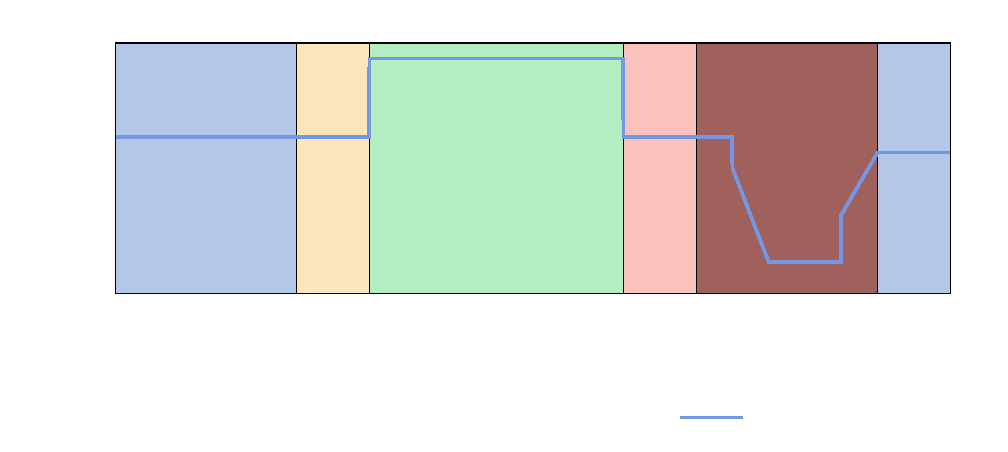
\includegraphics{Graphs/1/MiningSchedule/MiningSchedule}}%
    \gplfronttext
  \end{picture}%
\endgroup
}
		\caption[A typical operation schedule of a deep level mine.]{The typical operation schedule of a deep level mine \cite{Kriel2014Masters}.}
		\label{fig: Mining schedule}
	\end{figure}
	\paragraph*{Pneumatic rock drills}\leavevmode\\
	Compressed air is used to power pneumatic rock drills within a mine. These drills are heavy, hard to manoeuvre and  and inefficient \cite{van2008development}. However mines have widely adopted the use pneumatic drills for there reliability. \par
	Drilling is mainly performed in the production areas or stopes of a mine. The drills are used to drill holes into the rock face. Once the holes have been drilled, explosives are installed to break up the rock.\par
	A study by  Bester \textit{et al.} showed that between 2002 and 2013 compressed air and energy consumption per tonne of ore produced had steadily increased as shown in figure \ref{fig: Compressed energy and air flow per ton}. The increase in consumption per \gls{t} was a result of a reduction in air pressure at the mining stopes. Measurements indicated that the pressure was as low as 300 \gls{kpa}. This reduced the efficiency of the rock drills. Before 2002 pressure was maintained above 500 \gls{kpa} at the stopes.  The study showed that reducing pressure delivered to the drills will reduce the efficiency of the drill.\cite{bester2013effect} \par
		\begin{figure}[h]
		\centering
		\fbox{% GNUPLOT: LaTeX picture with Postscript
\begingroup
  \makeatletter
  \providecommand\color[2][]{%
    \GenericError{(gnuplot) \space\space\space\@spaces}{%
      Package color not loaded in conjunction with
      terminal option `colourtext'%
    }{See the gnuplot documentation for explanation.%
    }{Either use 'blacktext' in gnuplot or load the package
      color.sty in LaTeX.}%
    \renewcommand\color[2][]{}%
  }%
  \providecommand\includegraphics[2][]{%
    \GenericError{(gnuplot) \space\space\space\@spaces}{%
      Package graphicx or graphics not loaded%
    }{See the gnuplot documentation for explanation.%
    }{The gnuplot epslatex terminal needs graphicx.sty or graphics.sty.}%
    \renewcommand\includegraphics[2][]{}%
  }%
  \providecommand\rotatebox[2]{#2}%
  \@ifundefined{ifGPcolor}{%
    \newif\ifGPcolor
    \GPcolortrue
  }{}%
  \@ifundefined{ifGPblacktext}{%
    \newif\ifGPblacktext
    \GPblacktextfalse
  }{}%
  % define a \g@addto@macro without @ in the name:
  \let\gplgaddtomacro\g@addto@macro
  % define empty templates for all commands taking text:
  \gdef\gplbacktext{}%
  \gdef\gplfronttext{}%
  \makeatother
  \ifGPblacktext
    % no textcolor at all
    \def\colorrgb#1{}%
    \def\colorgray#1{}%
  \else
    % gray or color?
    \ifGPcolor
      \def\colorrgb#1{\color[rgb]{#1}}%
      \def\colorgray#1{\color[gray]{#1}}%
      \expandafter\def\csname LTw\endcsname{\color{white}}%
      \expandafter\def\csname LTb\endcsname{\color{black}}%
      \expandafter\def\csname LTa\endcsname{\color{black}}%
      \expandafter\def\csname LT0\endcsname{\color[rgb]{1,0,0}}%
      \expandafter\def\csname LT1\endcsname{\color[rgb]{0,1,0}}%
      \expandafter\def\csname LT2\endcsname{\color[rgb]{0,0,1}}%
      \expandafter\def\csname LT3\endcsname{\color[rgb]{1,0,1}}%
      \expandafter\def\csname LT4\endcsname{\color[rgb]{0,1,1}}%
      \expandafter\def\csname LT5\endcsname{\color[rgb]{1,1,0}}%
      \expandafter\def\csname LT6\endcsname{\color[rgb]{0,0,0}}%
      \expandafter\def\csname LT7\endcsname{\color[rgb]{1,0.3,0}}%
      \expandafter\def\csname LT8\endcsname{\color[rgb]{0.5,0.5,0.5}}%
    \else
      % gray
      \def\colorrgb#1{\color{black}}%
      \def\colorgray#1{\color[gray]{#1}}%
      \expandafter\def\csname LTw\endcsname{\color{white}}%
      \expandafter\def\csname LTb\endcsname{\color{black}}%
      \expandafter\def\csname LTa\endcsname{\color{black}}%
      \expandafter\def\csname LT0\endcsname{\color{black}}%
      \expandafter\def\csname LT1\endcsname{\color{black}}%
      \expandafter\def\csname LT2\endcsname{\color{black}}%
      \expandafter\def\csname LT3\endcsname{\color{black}}%
      \expandafter\def\csname LT4\endcsname{\color{black}}%
      \expandafter\def\csname LT5\endcsname{\color{black}}%
      \expandafter\def\csname LT6\endcsname{\color{black}}%
      \expandafter\def\csname LT7\endcsname{\color{black}}%
      \expandafter\def\csname LT8\endcsname{\color{black}}%
    \fi
  \fi
    \setlength{\unitlength}{0.0500bp}%
    \ifx\gptboxheight\undefined%
      \newlength{\gptboxheight}%
      \newlength{\gptboxwidth}%
      \newsavebox{\gptboxtext}%
    \fi%
    \setlength{\fboxrule}{0.5pt}%
    \setlength{\fboxsep}{1pt}%
\begin{picture}(9360.00,4032.00)%
    \gplgaddtomacro\gplbacktext{%
      \colorrgb{0.42,0.42,0.42}%
      \put(682,924){\makebox(0,0)[r]{\strut{}$0$}}%
      \colorrgb{0.42,0.42,0.42}%
      \put(682,1230){\makebox(0,0)[r]{\strut{}$5$}}%
      \colorrgb{0.42,0.42,0.42}%
      \put(682,1536){\makebox(0,0)[r]{\strut{}$10$}}%
      \colorrgb{0.42,0.42,0.42}%
      \put(682,1842){\makebox(0,0)[r]{\strut{}$15$}}%
      \colorrgb{0.42,0.42,0.42}%
      \put(682,2148){\makebox(0,0)[r]{\strut{}$20$}}%
      \colorrgb{0.42,0.42,0.42}%
      \put(682,2453){\makebox(0,0)[r]{\strut{}$25$}}%
      \colorrgb{0.42,0.42,0.42}%
      \put(682,2759){\makebox(0,0)[r]{\strut{}$30$}}%
      \colorrgb{0.42,0.42,0.42}%
      \put(682,3065){\makebox(0,0)[r]{\strut{}$35$}}%
      \colorrgb{0.42,0.42,0.42}%
      \put(682,3371){\makebox(0,0)[r]{\strut{}$40$}}%
      \colorrgb{0.42,0.42,0.42}%
      \put(814,704){\makebox(0,0){\strut{}$2002$}}%
      \colorrgb{0.42,0.42,0.42}%
      \put(2025,704){\makebox(0,0){\strut{}$2004$}}%
      \colorrgb{0.42,0.42,0.42}%
      \put(3237,704){\makebox(0,0){\strut{}$2006$}}%
      \colorrgb{0.42,0.42,0.42}%
      \put(4448,704){\makebox(0,0){\strut{}$2008$}}%
      \colorrgb{0.42,0.42,0.42}%
      \put(5659,704){\makebox(0,0){\strut{}$2010$}}%
      \colorrgb{0.42,0.42,0.42}%
      \put(6871,704){\makebox(0,0){\strut{}$2012$}}%
      \colorrgb{0.42,0.42,0.42}%
      \put(8082,704){\makebox(0,0){\strut{}$2014$}}%
      \colorrgb{0.42,0.42,0.42}%
      \put(8214,924){\makebox(0,0)[l]{\strut{}$0$}}%
      \colorrgb{0.42,0.42,0.42}%
      \put(8214,1230){\makebox(0,0)[l]{\strut{}$50$}}%
      \colorrgb{0.42,0.42,0.42}%
      \put(8214,1536){\makebox(0,0)[l]{\strut{}$100$}}%
      \colorrgb{0.42,0.42,0.42}%
      \put(8214,1842){\makebox(0,0)[l]{\strut{}$150$}}%
      \colorrgb{0.42,0.42,0.42}%
      \put(8214,2148){\makebox(0,0)[l]{\strut{}$200$}}%
      \colorrgb{0.42,0.42,0.42}%
      \put(8214,2453){\makebox(0,0)[l]{\strut{}$250$}}%
      \colorrgb{0.42,0.42,0.42}%
      \put(8214,2759){\makebox(0,0)[l]{\strut{}$300$}}%
      \colorrgb{0.42,0.42,0.42}%
      \put(8214,3065){\makebox(0,0)[l]{\strut{}$350$}}%
      \colorrgb{0.42,0.42,0.42}%
      \put(8214,3371){\makebox(0,0)[l]{\strut{}$400$}}%
    }%
    \gplgaddtomacro\gplfronttext{%
      \csname LTb\endcsname%
      \put(176,2147){\rotatebox{-270}{\makebox(0,0){\strut{}kWh/t}}}%
      \put(8851,2147){\rotatebox{-270}{\makebox(0,0){\strut{}$m^3$/t}}}%
      \put(4448,374){\makebox(0,0){\strut{}Year}}%
      \put(4448,3701){\makebox(0,0){\strut{}Compressed air energy and Volume consumed per ton}}%
      \csname LTb\endcsname%
      \put(3593,173){\makebox(0,0)[r]{\strut{}Energy per Ton (kWh/t)}}%
      \csname LTb\endcsname%
      \put(7352,173){\makebox(0,0)[r]{\strut{}Volume per Ton ($m^3$/t)}}%
    }%
    \gplbacktext
    \put(0,0){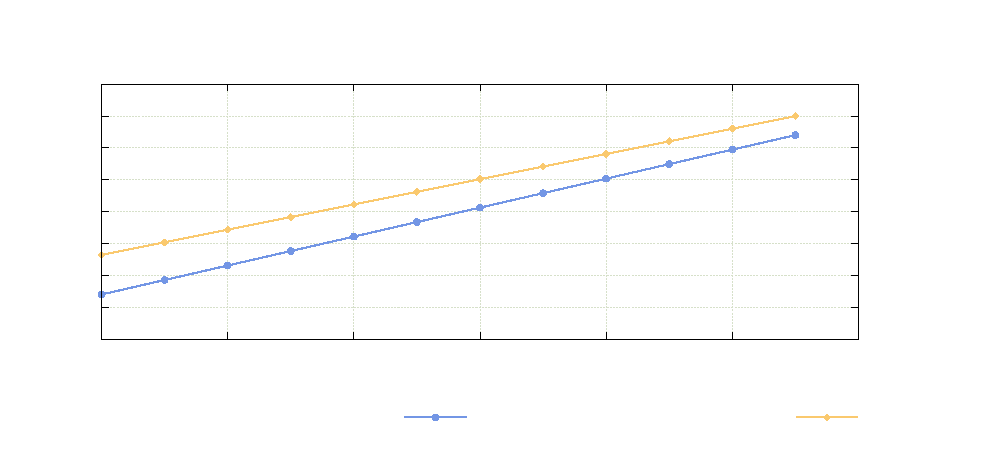
\includegraphics{Graphs/1/EVperT/EVperT}}%
    \gplfronttext
  \end{picture}%
\endgroup
}
		\caption[The Compressed air energy and flow consumed per T of ore produced.]{The Compressed air energy and flow consumed per T of ore produced. Adopted from Bester \textit{et al.} \cite{bester2013effect}.}
		\label{fig: Compressed energy and air flow per ton}
	\end{figure}

\paragraph*{Refuge bays}\leavevmode\\
Refuge bays are installed in mines to provide safety to miners during emergencies. Most mines will utilise compressed air to deliver safe, cool air to the refuge bay. The provision of 1.42 $l/s$ of air per person at a pressure between 200 and 300 \gls{kpa} is required to provide oxygen and prevent any poisonousness gas entering the refuge \cite{brake1999criteria}.\par
Airflow in the refuge bays can be controlled with a manual valve within the chamber. Any many cases, this valve is often misused by mine workers who open the valves fully in order to cool the bay through the decompression of the air. \texttt{*** need source ***}
\paragraph*{Compressed air control}\leavevmode\\
On many large compressed air networks, the intake guide vain position on a compressor is manipulated in order to obtain the air flow and pressure requirements. Typically, guide vains are opened and closed to increase and decrease the compressors discharge pressure. When more pressure is required than can be obtained with the guide vains fully opened, another compressor is needed to operate.\par
 As shown in the figure \ref{fig: Guide vain position}, showing guide vain positions vs power for a typical mining compressor, the guide vains are controlled between 40\% and 100\% of their fully open position. Reducing and increasing the guide vain position will effect the power output of the compressor.The relationship between power and guide vain position of a compressor can be approximated as a linear function. A guide vain position of 40\% will relate to an output power of about 60\% of maximum power.
 	\begin{figure}[h]
 	\centering
 	\fbox{% GNUPLOT: LaTeX picture with Postscript
\begingroup
  \makeatletter
  \providecommand\color[2][]{%
    \GenericError{(gnuplot) \space\space\space\@spaces}{%
      Package color not loaded in conjunction with
      terminal option `colourtext'%
    }{See the gnuplot documentation for explanation.%
    }{Either use 'blacktext' in gnuplot or load the package
      color.sty in LaTeX.}%
    \renewcommand\color[2][]{}%
  }%
  \providecommand\includegraphics[2][]{%
    \GenericError{(gnuplot) \space\space\space\@spaces}{%
      Package graphicx or graphics not loaded%
    }{See the gnuplot documentation for explanation.%
    }{The gnuplot epslatex terminal needs graphicx.sty or graphics.sty.}%
    \renewcommand\includegraphics[2][]{}%
  }%
  \providecommand\rotatebox[2]{#2}%
  \@ifundefined{ifGPcolor}{%
    \newif\ifGPcolor
    \GPcolortrue
  }{}%
  \@ifundefined{ifGPblacktext}{%
    \newif\ifGPblacktext
    \GPblacktextfalse
  }{}%
  % define a \g@addto@macro without @ in the name:
  \let\gplgaddtomacro\g@addto@macro
  % define empty templates for all commands taking text:
  \gdef\gplbacktext{}%
  \gdef\gplfronttext{}%
  \makeatother
  \ifGPblacktext
    % no textcolor at all
    \def\colorrgb#1{}%
    \def\colorgray#1{}%
  \else
    % gray or color?
    \ifGPcolor
      \def\colorrgb#1{\color[rgb]{#1}}%
      \def\colorgray#1{\color[gray]{#1}}%
      \expandafter\def\csname LTw\endcsname{\color{white}}%
      \expandafter\def\csname LTb\endcsname{\color{black}}%
      \expandafter\def\csname LTa\endcsname{\color{black}}%
      \expandafter\def\csname LT0\endcsname{\color[rgb]{1,0,0}}%
      \expandafter\def\csname LT1\endcsname{\color[rgb]{0,1,0}}%
      \expandafter\def\csname LT2\endcsname{\color[rgb]{0,0,1}}%
      \expandafter\def\csname LT3\endcsname{\color[rgb]{1,0,1}}%
      \expandafter\def\csname LT4\endcsname{\color[rgb]{0,1,1}}%
      \expandafter\def\csname LT5\endcsname{\color[rgb]{1,1,0}}%
      \expandafter\def\csname LT6\endcsname{\color[rgb]{0,0,0}}%
      \expandafter\def\csname LT7\endcsname{\color[rgb]{1,0.3,0}}%
      \expandafter\def\csname LT8\endcsname{\color[rgb]{0.5,0.5,0.5}}%
    \else
      % gray
      \def\colorrgb#1{\color{black}}%
      \def\colorgray#1{\color[gray]{#1}}%
      \expandafter\def\csname LTw\endcsname{\color{white}}%
      \expandafter\def\csname LTb\endcsname{\color{black}}%
      \expandafter\def\csname LTa\endcsname{\color{black}}%
      \expandafter\def\csname LT0\endcsname{\color{black}}%
      \expandafter\def\csname LT1\endcsname{\color{black}}%
      \expandafter\def\csname LT2\endcsname{\color{black}}%
      \expandafter\def\csname LT3\endcsname{\color{black}}%
      \expandafter\def\csname LT4\endcsname{\color{black}}%
      \expandafter\def\csname LT5\endcsname{\color{black}}%
      \expandafter\def\csname LT6\endcsname{\color{black}}%
      \expandafter\def\csname LT7\endcsname{\color{black}}%
      \expandafter\def\csname LT8\endcsname{\color{black}}%
    \fi
  \fi
    \setlength{\unitlength}{0.0500bp}%
    \ifx\gptboxheight\undefined%
      \newlength{\gptboxheight}%
      \newlength{\gptboxwidth}%
      \newsavebox{\gptboxtext}%
    \fi%
    \setlength{\fboxrule}{0.5pt}%
    \setlength{\fboxsep}{1pt}%
\begin{picture}(9360.00,4032.00)%
    \gplgaddtomacro\gplbacktext{%
      \colorrgb{0.00,0.00,0.00}%
      \put(814,704){\makebox(0,0)[r]{\strut{}$0$}}%
      \colorrgb{0.00,0.00,0.00}%
      \put(814,1214){\makebox(0,0)[r]{\strut{}$20$}}%
      \colorrgb{0.00,0.00,0.00}%
      \put(814,1725){\makebox(0,0)[r]{\strut{}$40$}}%
      \colorrgb{0.00,0.00,0.00}%
      \put(814,2235){\makebox(0,0)[r]{\strut{}$60$}}%
      \colorrgb{0.00,0.00,0.00}%
      \put(814,2746){\makebox(0,0)[r]{\strut{}$80$}}%
      \colorrgb{0.00,0.00,0.00}%
      \put(814,3256){\makebox(0,0)[r]{\strut{}$100$}}%
      \colorrgb{0.00,0.00,0.00}%
      \put(814,3767){\makebox(0,0)[r]{\strut{}$120$}}%
      \colorrgb{0.00,0.00,0.00}%
      \put(946,484){\makebox(0,0){\strut{}$0$}}%
      \colorrgb{0.00,0.00,0.00}%
      \put(2282,484){\makebox(0,0){\strut{}$20$}}%
      \colorrgb{0.00,0.00,0.00}%
      \put(3618,484){\makebox(0,0){\strut{}$40$}}%
      \colorrgb{0.00,0.00,0.00}%
      \put(4954,484){\makebox(0,0){\strut{}$60$}}%
      \colorrgb{0.00,0.00,0.00}%
      \put(6290,484){\makebox(0,0){\strut{}$80$}}%
      \colorrgb{0.00,0.00,0.00}%
      \put(7626,484){\makebox(0,0){\strut{}$100$}}%
      \colorrgb{0.00,0.00,0.00}%
      \put(8962,484){\makebox(0,0){\strut{}$120$}}%
    }%
    \gplgaddtomacro\gplfronttext{%
      \csname LTb\endcsname%
      \put(176,2235){\rotatebox{-270}{\makebox(0,0){\strut{}Output power (\%)}}}%
      \put(4954,154){\makebox(0,0){\strut{}Guide Vain Position (\%)}}%
    }%
    \gplbacktext
    \put(0,0){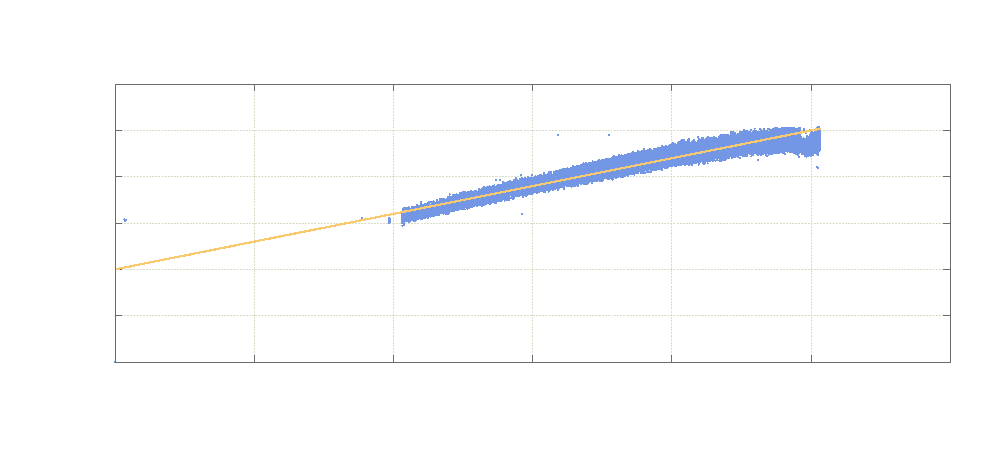
\includegraphics{Graphs/1/GuideVainPosition/GuideVainPosition}}%
    \gplfronttext
  \end{picture}%
\endgroup
}
 	\caption[The relation between guide vain position and compressor output power.]{The relation between guide vain position and compressor output power.}
 	\label{fig: Guide vain position}
 \end{figure}
 
	\subsection{Characteristic inefficiencies}
	As large compressed air distribution networks in the mining industry consist of multiple compressors with working areas up to eight kilometres away from the source \cite{Marais2012PhD}. The systems are prone to energy losses due to various characteristic inefficiencies. \par 
	Compressed air leakage accounts for as much as 35\% of the energy losses of a compressed air network \cite{Lawrence2004Improving}. Other systemic losses include, faulty valves, pipe diameter fluctuations, obstructed air compressor intake filters and inefficient compressors. \par
	\subsection{Instrumentation and measurements}
	For large industrial systems, instrumentation is necessary in order to control and monitor performance. In a large compressed air network, typical instrumentation	include digital and analog sensors, alarms, meters and  \glspl{plc}. Typically a \gls{scada} is installed in order to observe and monitor the instrumentation. 
	\subsection{Inefficiency identification methods}
	\texttt{Methods currently used by industry to identify and estimate losses due to an inefficiency}
	
	
\section{Simulations in industry}

Continuous improvements in computing hardware has led to major advancement in software technology. Consequently the use of computational simulation has become an increasingly valuable tool for many industries.\cite{kocsis2003integration} \par 

 In \textit{ Handbook of simulation: principles, methodology, advances, applications, and practice}, the advantages of the use of simulation in industry are discussed as follows \cite{banks1998handbook}: 
\begin{itemize}
	\item The ability to test new policies, operating procedures and methods without causing a disruption to the actual system.
	\item The means to identify problems in complex systems by gathering insight in the interactions within the system.
	\item The facility to compress or expand time to investigate phenomena thoroughly.
	\item The capability to determine the limits and constraints within a system.
	\item The potential to build consensus with regard to proposed designs or modifications.
\end{itemize}

\subsection{Thermal-hydraulic simulation}
\gls{ths} is the modelling and computational analysis of Thermal-hydraulic systems. \gls{ths} models can be developed large mining systems such as cooling ,compressed air water reticulation etc..\par
In industry, various software packages are used for modelling and simulating these systems. Two such packages are KY-pipe and Simulation Toolbox.
\texttt{STB background.}
\paragraph{KY Pipe}\leavevmode\\
\texttt{KY Pipe background.}
\paragraph{Simulation toolbox}\leavevmode\\
v\texttt{STB background.}
\section{Problem statement and objectives}
\texttt{Identification of research problem and formulation of objectives should be unambiguous and intelligible}
\subsection{Problem statement}
\subsection{Research objectives}

\section{Dissertation overview}
\texttt{Describe (in approximately one sentence each) the contents of each of the dissertation chapters. No results here.}